%
% GNU courseware, XIN YUAN, 2017
%

\documentclass[11pt]{beamer}
\usepackage{beamerthemesplit}
\usepackage{graphicx}
\usepackage{colortbl}
\usepackage[BoldFont,SlantFont,CJKchecksingle]{xeCJK}
\setCJKmainfont[BoldFont=SimHei,SlantedFont=KaiTi]{SimSun}
\setCJKsansfont[BoldFont=SimHei,SlantedFont=KaiTi]{SimSun}
\setCJKmonofont[ItalicFont={Adobe Fangsong Std}]{SimSun}
\setCJKfamilyfont{zhsong}{SimSun}
%\setCJKfamilyfont{zhhei}{Adobe Song Std}
\setCJKfamilyfont{zhhei}{SimHei}
%\setCJKfamilyfont{zhhei}{Adobe Heiti Std}
\setCJKfamilyfont{zhkai}{KaiTi}
\setCJKfamilyfont{zhfs}{FangSong}
\setCJKfamilyfont{zhls}{LiSu}
\setCJKfamilyfont{zhyy}{YouYuan}
\usetheme{warsaw}

\parindent 2em

%title
\title{生物智能与算法}
\author{袁昕}
\date{\today}

\begin{document}

%title
\frame{\titlepage}

\frame{
\centerline{\textbf{\Huge{课程介绍}}}
}

%tables

\section*{大纲}

\frame{\tableofcontents}

%introduction

\section{简介}
\subsection{定义}

\frame{\frametitle{简介}
计算智能也被称作“软计算”,是根据自然界生物体系的原理和规律,
模仿设计出具有记忆、学习、适应等特性的求解算法的总称。

~

这些算法通过计算机模拟,再现了生物的某些智能行为。
}

\subsection{历史}

\frame{\frametitle{历史}
	\begin{enumerate}
		\item<1-> 早期探索阶段(1995年之前)。
		\item<2-> 成型阶段(1995年-2000年)。
		\item<3-> 发展阶段(2001年-2010年)。
		\item<4-> 成熟阶段(2011年以来)。
	\end{enumerate}
}

\frame{\frametitle{历史-早期探索}
这一阶段虽然没有产生具有标志性的生物智能优化算法,但是却为后来的持续快速发展奠定了坚实的基础。
}

\frame{\frametitle{历史-成型}
在探索阶段的基础上一些生物智能优化算法开始设计成型。这一时期产生了三个非常经典的生物智能优化算法,
即由Kennedy和Eberhart于1995年提出的粒子群优化算法、
由Storn和Price于1997年提出的差分进化算法以及由Shi和Eberhart于1998年提出的基于惯性权重的粒子群优化算法。
粒子群优化算法是受鸟类的觅食行为的激励而提出的;差分进化算法是受生物进化过程的激励而提出的。
需要注意的是,这一阶段产生的生物智能优化算法的数量是比较少的。
但是,这一阶段产生的算法的设计框架一直被沿用至今。
}

\frame{\frametitle{历史-发展}
相较于成型阶段,发展阶段所产出的生物智能优化算法的数量显著增加。
这意味着生物智能优化算法在探索阶段和成型阶段的基础上开始逐渐走向成熟。
这一阶段也产生了非常具有代表性的算法,比如布谷鸟搜索算法和生物地理学优化算法。
布谷鸟搜索算法是受一些布谷鸟繁殖行为的启发而提出的;
生物地理学优化算法是受生物的迁徙现象的激励而提出的。
布谷鸟搜索算法首次引入了莱维飞行机制来增强全局搜索能力。
受此启发,现在很多学者已经把莱维飞行作为一种提升生物智能优化算法搜索性能的改进技术。
生物地理学优化算法得益于其设计的算法结构,具有较强的局部搜索能力。
因而,生物地理学优化算法经常与其它算法混合以获取更具竞争力的算法,
比如生物地理学优化算法与灰狼优化算法的混合、
生物地理学优化算法与布谷鸟搜索算法的混合以及生物地理学优化算法与粒子群优化算法的混合。
}

\frame{\frametitle{历史-成熟}
得益于前面三个阶段的积累,自2011年以来,大量的生物智能优化算法相继被学者们提出。
此外,值得一提是,在这一阶段,学者们采用生物智能优化算法成功地解决了许多不同类型的实际工程问题。
这表明生物智能优化算法的发展已经进入了较为成熟的阶段。
这一阶段也产生了许多代表性的生物智能优化算法,比如回溯搜索算法和教与学优化算法。
回溯搜索算法首次将历史种群用于指导产生下一代种群,并将服从标准正态分布的随机数引入到元启发式算法的设计中;
而教与学优化算法仅需要必需参数,即种群大小和终止条件,来执行搜索操作。
}

%methods

\section{方法}

\frame{\frametitle{方法}
	\begin{itemize}
		\item<1-> 进化(演化)算法(遗传算法,协同进化)
		\item<2-> 免疫算法
		\item<3-> 群集智能(蚁群算法,粒子群算法,飞鸟,鱼群,布谷鸟,蝙蝠,萤火虫)
		\item<4-> 模拟退火(源自物理,引出神经网络)
		\item<5-> 人工神经网络(连接型,模糊粗糙,记忆型,脉冲耦合,机器学习,深度)
	\end{itemize}
}

\frame{\frametitle{方法}
	\begin{itemize}
		\item<1-> 专家系统
		\item<2-> 生态动力系统
		\item<3-> 复杂网络和动力学
	\end{itemize}
}

\frame{\frametitle{方法}
都是\textsl{仿生算法}。

~

其最大特点就是不需要建立问题本身精确的数学模型,
适合于解决那些因为难以建立有效的形式化模型而用传统人工智能技术
又难以有效解决甚至无法解决的问题。
}

\frame{\frametitle{按激励源分类}
	\begin{enumerate}
		\item<1-> 受生物进化现象激励的智能优化算法。
这类算法是受自然界中生物的进化过程的启发而提出的,比如经典的差分进化算法和遗传算法;
		\item<2-> 受动物的日常行为激励的智能优化算法。
这类算法是受动物的觅食、围猎以及求偶等行为的启发而提出的,比如粒子群优化算法、布谷鸟搜索算法和灰狼优化算法等等;
		\item<3-> 受植物的习性激励的智能优化算法,比如杂草优化算法;
		\item<4-> 受人类活动激励的智能优化算法,比如排队搜索算法、人工神经网络算法以及教与学优化算法等;
		\item<5-> 受自然界中的物理现象激励的智能优化算法,比如水循环算法、重力搜索算法等。
	\end{enumerate}
}

\frame{\frametitle{按参数类型分类}
	\begin{enumerate}
		\item<1-> 必需参数。
指任何一个生物智能优化算法都需要的,其包括种群大小和终止条件(比如最大迭代次数和最大函数迭代次数等)。
比如教与学优化算法、人工神经网络算法等;
		\item<2-> 控制参数。
指除了必需参数之外反映算法特征的参数,比如差分进化算法中的缩放因子和交叉率、粒子群优化算法中的惯性权重和学习因子、布谷鸟搜索算法中的发现概率等。
	\end{enumerate}
}

\frame{\frametitle{优点}

{\CJKfamily{zhfs}
智能计算具有简单、通用、鲁棒性强、适于并行处理的优点,
使其在并行搜索、联想记忆、模式识别、知识自动获取等方面得到了广泛的应用。
}

~

本课目的之一,要能说出各种方法的\textbf{本质}和\textbf{思维共性}。
}

\frame{\frametitle{缺点}

本课目的之一,要能说出每种方法的假设、缺点和适用范围。
}

\frame{\frametitle{与传统人工智能对比}

{\CJKfamily{zhhei}
计算智能有别于传统的符号智能。符号智能是以知识为基础,通过推理进行问题求解,也即传统的人工智能;
而计算智能则是以数据为基础,通过训练建立联系,进行问题求解。
}

~

{\CJKfamily{zhkai}
计算智能是以联接主义为主的思维方式,即研究简单个体如何在简单交互规则指导下,
构成具有复杂智能行为的高层系统。
}

~

数据驱动,研究以相关性为主,因果性为辅。这二者分别对应着定性解释和定量解释。概率统计是其基本工具。
}

\frame{\frametitle{现状}
由于过于强调仿生,导致现在的研究针对每一种前人未述及的动物行为就发表大量论文,形成了滥觞。
在研究范式上停滞不前。
}

\frame{\frametitle{挑战}
\begin{enumerate}
\item<1-> 无免费午餐理论
\item<2-> 参数设置
\end{enumerate}
}

\frame{\frametitle{挑战-无免费午餐理论}

一个优化算法在一个具体问题上能够获取理想的解决方案,
并不意味着这一优化算法也能够在其它问题上取得理想的解决方案。
简而言之,依据“无免费午餐理论”,不存在能够解决所有优化问题的算法。
也就是说,一个算法在求解一类问题上的成功不能保证这种算法也能在其它类型的问题上得到理想的解决方案。
不同类型的优化问题通常具有不同的特点,比如变量的多少、目标函数的复杂程度以及约束条件的松紧等,
这是支持无免费午餐理论的基础。
}

\frame{\frametitle{挑战-无免费午餐理论}
例子1:

~

综合学习的粒子群优化算法是粒子群优化算法的一个非常经典的改进版本。
作者采用16个基准测试函数检验所提出的综合学习的粒子群优化算法的性能。
依据实验结果,当基准测试函数的维度为30时,综合学习的粒子群优化算法优于比较的算法在10个基准测试函数上,
而在其它6个基准测试函数上,综合学习的粒子群优化算法并没有取得最优的解
(Liang JJ, Qin AK, Suganthan PN, Baskar S.
Comprehensive learning particle swarm optimizer for global optimization of multimodal functions [J].
IEEE Transactions on Evolutionary Computation, 2006, 10(3): 281–295)
}

\frame{\frametitle{挑战-无免费午餐理论}
例子2:

~

集成粒子群优化算法是粒子群优化算法的一个改进版本。
作者用25个基准测试函数检验所提出的集成粒子群优化算法的性能。
依据实验结果,集成粒子群优化算法在19个基准测试函数上优于粒子群优化算法;
集成粒子群优化算法在4个基准测试函数上与粒子群优化算法具有相同的性能;
集成粒子群优化算法在2个基准测试函数上劣于粒子群优化算法
(Lynn N, Suganthan PN. Ensemble particle swarm optimizer [J].
Applied Soft Computing, 2017, 55: 533–548)
}

\frame{\frametitle{挑战-参数角度}
绝大部分群智能优化算法除了必需参数之外,都需要控制参数。
具有控制参数的群智能优化算法通常会面临一个难题:
在求解不同特点的优化问题时,如何设置它们的控制参数才能获取最优的解决方案?
假如控制参数设置得当,这些算法可以得到比较理想的解决方案;
否则,这些算法可能得到比较糟糕的解决方案。
显然,控制参数的设置将会制约群智能优化算法的应用潜力。
}

\frame{\frametitle{挑战-参数角度}
例子:

~

布谷鸟搜索算法中的一个非常重要的参数称为发现概率。
下图给出了布谷鸟搜索算法在两个不同测试函数上的性能,
从图(a)可以看到,对于sphere函数,最优的发现概率是0.25;
对于rosenbrock函数来说,最优的发现概率是0.05。

\begin{minipage}[b]{\textwidth}
\begin{figure}[hb]
\centering
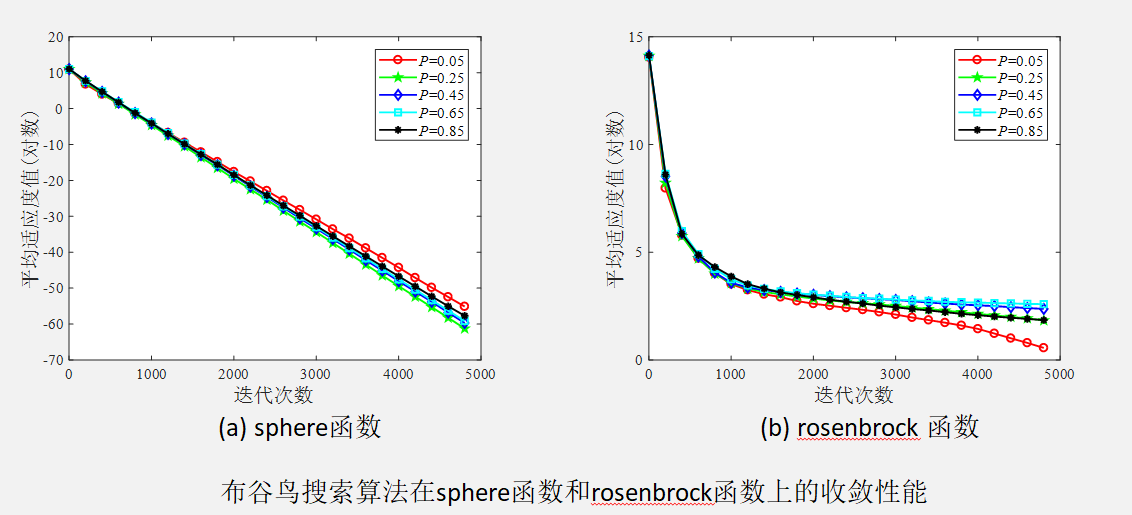
\includegraphics[width=0.8\textwidth]{0-files/qzn.png}
\end{figure}
\end{minipage}
}

\frame{\frametitle{挑战}
从理论角度来说,受“无免费午餐理论”和“参数困境”的激励,
设计更多简单、高效且仅需要必需参数的群智能优化算法,
以求解不同类型的优化问题。
}

\section{应用}

\frame{\frametitle{应用}

自80年代中后期以来计算智能在众多领域的科学家加入下得到了极大的发展。

~

\textcolor{blue}{看看有哪些应用领域?}
}

\frame{\frametitle{应用}
现实生产生活中,优化问题经常碰到,比如电力经济调度问题、机器人路径规划问题、图像分割问题、
时间序列预测问题等等。

~

工程角度看,优化问题就是具有不止一个可行解决方案的问题。
求解优化问题就是从众多可行方案中选择一个最理想的可行方案。
这个最理想的解决方案也称为全局最优解决方案。
}

\section{工作流程}

\frame{\frametitle{工作流程}
	\begin{enumerate}
		\item<1-> 清晰地描述问题
		\item<2-> 描述数据,识别变量,不变量和隐变量
		\item<3-> 探索量之间的关系,借鉴仿生系统,建立数学模型
		\item<4-> 数字实验和评价
		\item<5-> 对模型进行数学抽象和逻辑分析,给出假设
		\item<6-> 给出直观的几何意义和物理意义
		\item<7-> 和已有方法进行对比,给出优缺点和适用范围
		\item<8-> 撰写报告和论文
	\end{enumerate}
}

\section{课程报告}

\frame{\frametitle{课程报告}
	\begin{enumerate}
		\item 上课时各小组的幻灯或小报告
		\item 每位同学整理一份报告
			\begin{itemize}
				\item 对已有的一个方法的深入阐述,有余力的同学可编程实验并评价
				\item 探索新的方法
				\item 针对科研中的问题,提出计算智能方法并试验
			\end{itemize}
		\item 协作网址或报告发邮件给 yxxinyuan@zju.edu.cn
	\end{enumerate}
}

\frame{\frametitle{报告形式}
\begin{minipage}[t]{\textwidth}
幻灯和报告可充分应用图形摘要、漫画等趣味形式,形成既科普,又专业的作品。
\end{minipage}

\uncover<2->{
\begin{minipage}[b]{\textwidth}
\begin{figure}[hb]
\centering
\includegraphics[width=0.8\textwidth]{0-files/ant.png}
\end{figure}
\end{minipage}
}
}

\frame{\frametitle{算法对比}

\begin{table}[htbp]
\centering
\begin{tabular}{|l|c|r|}
\hline
算法   &  精度    &  运算时间(s)\\
\hline
蚁群   &  90\%    &  10.3\\
\hline
\rowcolor[rgb]{0.0, 0.8, 0.8}
进化   &  \textcolor[rgb]{1.0, 1.0, 0.0}{91.2\%}  &  20.6\\
\hline
免疫   &  93.1\%  &  15.9\\
\hline
\end{tabular}
\end{table}
}

\frame{\frametitle{口号}

\centerline{\textbf{\Huge{\textcolor[rgb]{0.5, 0.5, 0.0}{我们不做数学符号的搬运工!}}}}
}

\frame{\frametitle{结束}

\centerline{\textbf{\Huge{结束!}}}
}

\frame{\frametitle{版权申明}

本作品采用知识共享 署名-非商业性使用-禁止演绎 3.0 中国大陆 许可协议进行许可。
要查看该许可协议,可访问 http://creativecommons.org/licenses/by-nc-nd/3.0/cn/ 或者
写信到 Creative Commons, PO Box 1866, Mountain View, CA 94042, USA。
}

\end{document}
